\section{Part IV - State Estimation}\label{sec:part4}

\subsection{Problem 1 - State-space formulation}\label{subsec:P4p1}
We wish to derive a state-space formulation from the system of linearized equations derived in \ref{subsec:P1p2} on the form

\begin{equation}\label{eq:state-space}
\begin{split}
    \mathbf{\dot{x}} &= \mathbf{Ax + Bu}\\
    \mathbf{y} &= \mathbf{Cx}
\end{split}
\end{equation}
where \textbf{A, B} and \textbf{C} are matrices defined below. The state vector, the input vector and the output vector are now given by:

\begin{align}\label{eq:states_part4}
    \textbf{x} &= \begin{bmatrix} \tilde{p} \\ \dot{\tilde{p}} \\ \tilde{e} \\ \dot{\tilde{e}} \\ \tilde{\lambda} \\ \dot{\tilde{\lambda}} \end{bmatrix}, &\textbf{u} &= \begin{bmatrix} \tilde{V_{s}} \\ \tilde{V_{d}} \end{bmatrix}, &\mathbf{y} &= \begin{bmatrix} \tilde{p} \\ \tilde{e} \\ \tilde{\lambda} \end{bmatrix}
\end{align}
From the output equation and the state vector, we can directly see that the matrix \textbf{C} is given by 
\begin{equation}
    \mathbf{C} = 
    \begin{bmatrix}
    1 & 0 & 0 & 0 & 0 & 0 \\
    0 & 0 & 1 & 0 & 0 & 0 \\
    0 & 0 & 0 & 0 & 1 & 0
    \end{bmatrix}
\end{equation}
Furthermore, using the equations \eqref{eq:lin_model_pitch}-\eqref{eq:lin_model_travel}, the state equation can be written as
\begin{equation}\label{eq:state_matrices_P4p1}
    \mathbf{\dot{x}} = 
    \begin{bmatrix} 
        \dot{\tilde{p}} \\ 
        \ddot{\tilde{p}} \\ 
        \dot{\tilde{e}} \\ 
        \ddot{\tilde{e}} \\ 
        \dot{\tilde{\lambda}}\\ 
        \ddot{\tilde{\lambda}} 
    \end{bmatrix} = 
    \begin{bmatrix} 
        x_{2}\\ 
        K_1\tilde{V_d}\\ 
        x_4\\ 
        K_2\tilde{V_s}\\ 
        x_6\\ 
        K_3 x_1 
    \end{bmatrix} =
    \underbrace{
    \begin{bmatrix}
        0 & 1 & 0 & 0 & 0 & 0 \\
        0 & 0 & 0 & 0 & 0 & 0 \\
        0 & 0 & 0 & 1 & 0 & 0 \\
        0 & 0 & 0 & 0 & 0 & 0 \\
        0 & 0 & 0 & 0 & 0 & 1 \\
        K_3 & 0 & 0 & 0 & 0 & 0
    \end{bmatrix}}_\mathbf{A}\mathbf{x} + 
    \underbrace{
    \begin{bmatrix}
        0 & 0 \\
        0 & K_1 \\
        0 & 0 \\
        K_2 & 0 \\
        0 & 0 \\
        0 & 0 
    \end{bmatrix}}_\mathbf{B}\mathbf{u}
\end{equation}

\subsection{Problem 2 - Linear observer}\label{subsec:P4p2}
In order to examine the observability of the system, we calculate the observability matrix using
\begin{equation}\label{eq:obs_matrix}
    {\mathcal {O}}={\begin{bmatrix}C\\CA\\CA^{2}\\\vdots \\CA^{n-1}\end{bmatrix}}
\end{equation}
We have learned from\cite{Lecture_5} that the criteria for a system to be observable is that \eqref{eq:obs_matrix} has full rank. In our case, this is achieved after the two first computations in the observability matrix:
\begin{equation}\label{eq:obs_matrix_calc}
    {\mathcal {O}}_{2}=
    {\begin{bmatrix}
        1 & 0 & 0 & 0 & 0 & 0\\
        0 & 0 & 1 & 0 & 0 & 0\\
        0 & 0 & 0 & 0 & 1 & 0\\
        0 & 1 & 0 & 0 & 0 & 0\\
        0 & 0 & 0 & 1 & 0 & 0\\
        0 & 0 & 0 & 0 & 0 & 1
    \end{bmatrix}}
\end{equation}
Hence, our system is indeed observable.\\
\\
Next, we wish to create a linear observer for the system of the form:
\begin{equation}\label{observer_system}
    \mathbf{\dot{\hat{x}} = A\hat{x} + Bu + L(y - C\hat{x})}
\end{equation}
where \textbf{L} is the observer gain matrix.
Because the system is observable, we have the opportunity to place the poles of the system where we want in order to obtain an optimal response. We can do this by choosing an appropriate gain matrix \textbf{L}. The estimator $\mathbf{\hat{x}}$ has the same poles as $\mathbf{A - LC}$. Generally, we want the error dynamics to be faster than the system itself. In practice, this means that the poles of $\mathbf{A - LC}$ should be placed further into the left half plane than the poles of $\mathbf{A - BK}$, which represents the system dynamics. We place the estimator poles on a circular arc in the left half plane, shown in \cref{fig:Pole_placement_P4p2}. The radius of this arc is determined by a multiple of the distance to the most negative pole of the original system. MATLAB provides a simple function place() to compute the observer gain matrix \textbf{L}. MATLAB code for implementing this is shown in \cref{subsec:P4p2_init.m}.
\begin{figure}[htb]
	\centering
		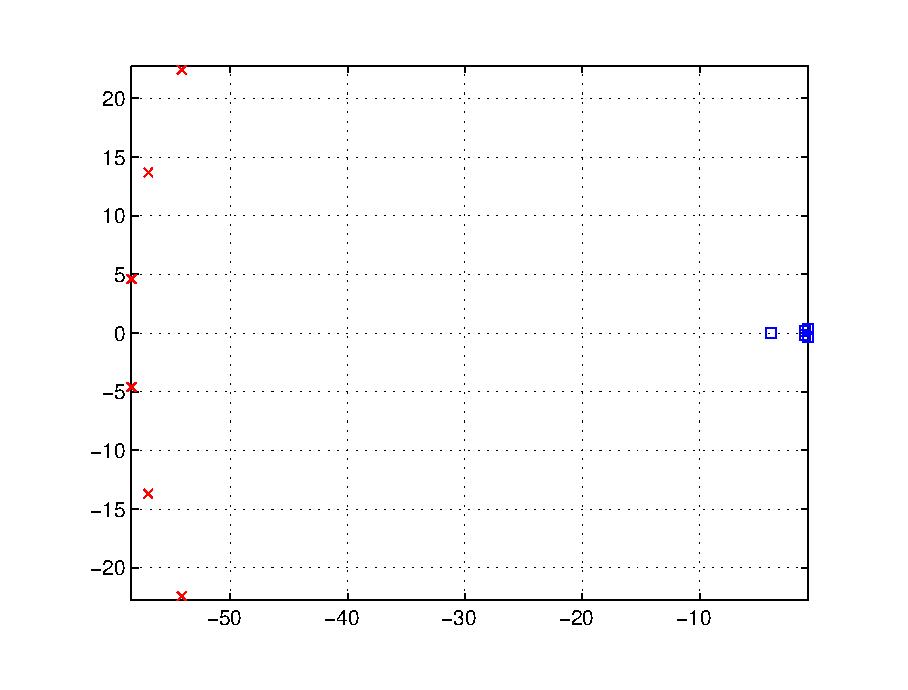
\includegraphics[width=0.8\textwidth]{figures/Pole_placement_P4p2_integral.eps}
	\caption{Pole placement for the system with integral controller from part III. The system poles are located in blue on the right, while the observer poles are seen in red.}
\label{fig:Pole_placement_P4p2}
\end{figure}
\\

Choosing a ideal gain matrix will be very important for this system, because although we want a fast estimator, the further into the left half plane the estimator poles are located, the more we will amplify noise in the measurements. In our project, we ended up placing the estimator poles on an arc with radius 13 times the distance of the most negative pole from the original system.\\
\\As in part 3, we tried tuning with different values for the matrices \textbf{Q} and \textbf{R} until the desired behaviour was reached. We seemed however to get the best results with similar values as in part III, see \cref{eq:P3_weighting_matrices}. With the computed gain matrix
\begin{equation}\label{eq:L_P4p2}
\mathbf{L} = \begin{bmatrix}
97,94 & 6,20 & -13,90\\
2476,40 & 318,65 & -725,98\\
-2,47 & 98,99 &	1,78\\
-114,14 & 2600,04 &	80,90\\
15,36 & 2,71 & 96,90\\
786,98 & -148,13 & 2412,86
\end{bmatrix}
\end{equation}
we were able to reach satisfying results with both controllers from part III. Plots of the estimated values versus the real values for both controllers are shown below, first for the regular P controller in \cref{fig:P4p2_states_vs_obs} and then the PI controller in \cref{fig:P4p2_int_states_vs_obs}. The Simulink-diagram to show the implementation of the observer is included in \cref{fig:P4_observer}, \cref{sec:simulink}
\subsection{Problem 3 - Observer without pitch}\label{subsec:P4p3}
We aim to control our system by only measuring $\tilde{e}$ and $\tilde{\lambda}$. The output \textbf{y} and output matrix \textbf{C} becomes:
\begin{equation}\label{eq:y_P4p3}
\mathbf{y} = 
\begin{bmatrix}
\tilde{e}\\
\tilde{\lambda}
\end{bmatrix}
\end{equation}
and
\begin{equation}\label{eq:C_P4p3}
\mathbf{C} = 
    \begin{bmatrix}
    0 & 0 & 1 & 0 & 0 & 0 \\
    0 & 0 & 0 & 0 & 1 & 0 
    \end{bmatrix}
\end{equation}
Again, as in \ref{subsec:P4p2}, we use \eqref{eq:obs_matrix} to examine if the system is observable:
\begin{equation}\label{eq:obs_matrix_calc_last}
    \mathcal {O}=
    {\begin{bmatrix}
        0 & 0 & 1 & 0 & 0 & 0\\
        0 & 0 & 0 & 0 & 1 & 0\\
        0 & 0 & 0 & 1 & 0 & 0\\
        0 & 0 & 0 & 0 & 0 & 1\\
        0 & 0 & 0 & 0 & 0 & 0\\
        -K_3 & 0 & 0 & 0 & 0 & 0\\
        0 & 0 & 0 & 0 & 0 & 0\\
        0 & -K_3 & 0 & 0 & 0 & 0\\
        0 & 0 & 0 & 0 & 0 & 0\\
        0 & 0 & 0 & 0 & 0 & 0\\
        0 & 0 & 0 & 0 & 0 & 0\\
        0 & 0 & 0 & 0 & 0 & 0
    \end{bmatrix}}
\end{equation}
We can clearly see that \eqref{eq:obs_matrix_calc_last} has full rank, so the system is observable when measuring only $\tilde{e}$ and $\tilde{\lambda}$. However, if one only measures $\tilde{p}$ and $\tilde{e}$, this is not the case! The output matrix becomes:
\begin{equation}\nonumber
\mathbf{C} = 
    \begin{bmatrix}
    1 & 0 & 0 & 0 & 0 & 0 \\
    0 & 0 & 1 & 0 & 0 & 0 
    \end{bmatrix},
\end{equation}
which leads to the observability matrix
\begin{equation}\nonumber
    \mathcal {O}=
    {\begin{bmatrix}
        1 & 0 & 0 & 0 & 0 & 0\\
        0 & 0 & 1 & 0 & 0 & 0\\
        0 & 1 & 0 & 0 & 0 & 0\\
        0 & 0 & 0 & 1 & 0 & 0\\
        0 & 0 & 0 & 0 & 0 & 0\\
        0 & 0 & 0 & 0 & 0 & 0\\
        0 & 0 & 0 & 0 & 0 & 0\\
        0 & 0 & 0 & 0 & 0 & 0\\
        0 & 0 & 0 & 0 & 0 & 0\\
        0 & 0 & 0 & 0 & 0 & 0\\
        0 & 0 & 0 & 0 & 0 & 0\\
        0 & 0 & 0 & 0 & 0 & 0
    \end{bmatrix}}
\end{equation}
Now, the observability matrix has rank 4, which is not full rank. Hence the system is not observable and it will be impossible to control with a state estimator. This is due to the fact that the pitch, $\tilde{p}$, can be found by differentiating $\tilde{\lambda}$ twice and multiplying with a constant $K_3$, \eqref{eq:lin_model_travel}. However, this is not the case when we try to replace $\tilde{\lambda}$ with $\tilde{p}$ as a measured state. If we try to integrate $\tilde{\lambda}$ twice in order to find the pitch, we will end up with unknown constants, and thus information will be lost.\\
\\
When testing the helicopter with \eqref{eq:y_P4p3} as the measured states, it turned out to be difficult to acquire a good response. Even though it is possible in theory to control the system with only these two measured states, it did not work well in practice, as we can see from \cref{fig:P4p3}. This can be explained by the fact that we differentiate $\tilde{\lambda}$ three times to get the pitch rate $\dot{\tilde{p}}$. During this action we also differentiate measurement noise, which results in a significant amplification of this noise. After some testing, we chose the estimator poles to be on the real axis, and much lower values of L compared to \eqref{eq:L_P4p2}:
\begin{equation}\nonumber
\mathbf{L} = \begin{bmatrix}
1,95 & -90,72\\
1,19 & -44,14\\
6,50 & -0,01\\
10,00 &	-0,012\\
-0,07 &	10,50\\
-0,54 &	38,00
\end{bmatrix}
\end{equation}
This will lead to a slower observer, but less amplification of noise, and by placing poles on the real axis, we achieve as much damping as possible. After tuning of the weighting matrices, we found a somewhat acceptable behaviour when reducing the integral effect by giving the last two diagonal elements of the weighting matrix \textbf{Q} small values, and making power less available by increasing values of \textbf{R}. We ended up with the following matrices:
\begin{align}\nonumber
&\mathbf{Q} = 
\begin{bmatrix}
    8 & 0 & 0 & 0 & 0\\
    0 & 4 & 0 & 0 & 0\\
    0 & 0 & 50 & 0 & 0\\
    0 & 0 & 0 & 0.01 & 0\\
    0 & 0 & 0 & 0 & 0.01
\end{bmatrix},
&\mathbf{R} =
\begin{bmatrix}
    1000 & 0\\
    0 & 1000
\end{bmatrix},
\end{align}
\begin{equation}\nonumber
\mathbf{K} =
\begin{bmatrix}
    0 & 0 & 0.3149 & 0 & 0.0032\\
    0.1090 & 0.6124 & 0 & 0.0032 & 0
\end{bmatrix}.
\end{equation}
\begin{figure}[htb]
	\centering
		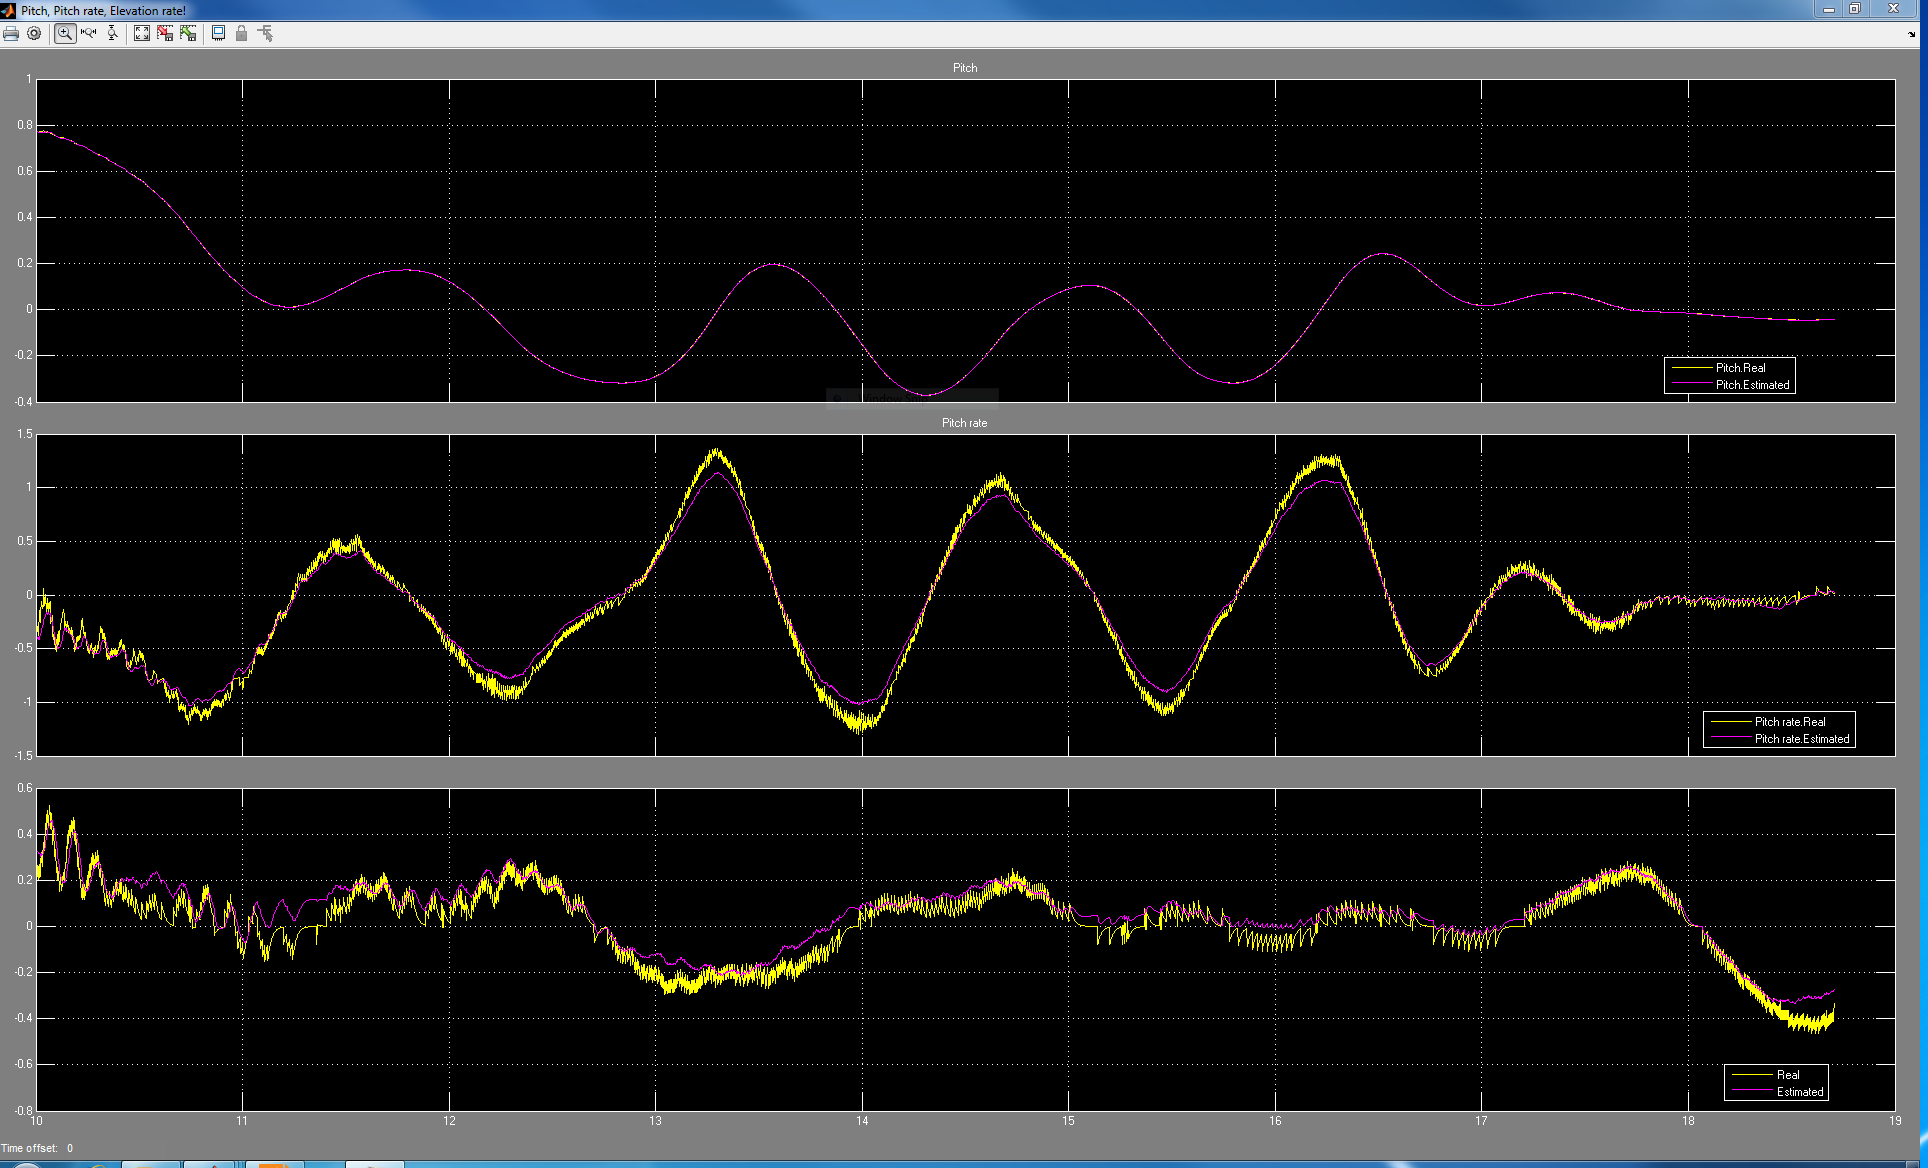
\includegraphics[width=1\textwidth]{figures/superplots_P4p2_del1_best_husk_ratenavn.PNG}
	\caption{Part IV, problem 2 - P controller. Shows the real (yellow) and estimated (purple) states for pitch, pitch rate and elevation rate respectively. As we can see, the estimated states follows the real states quite well.}
\label{fig:P4p2_states_vs_obs}
\end{figure}
\begin{figure}[htb]
	\centering
		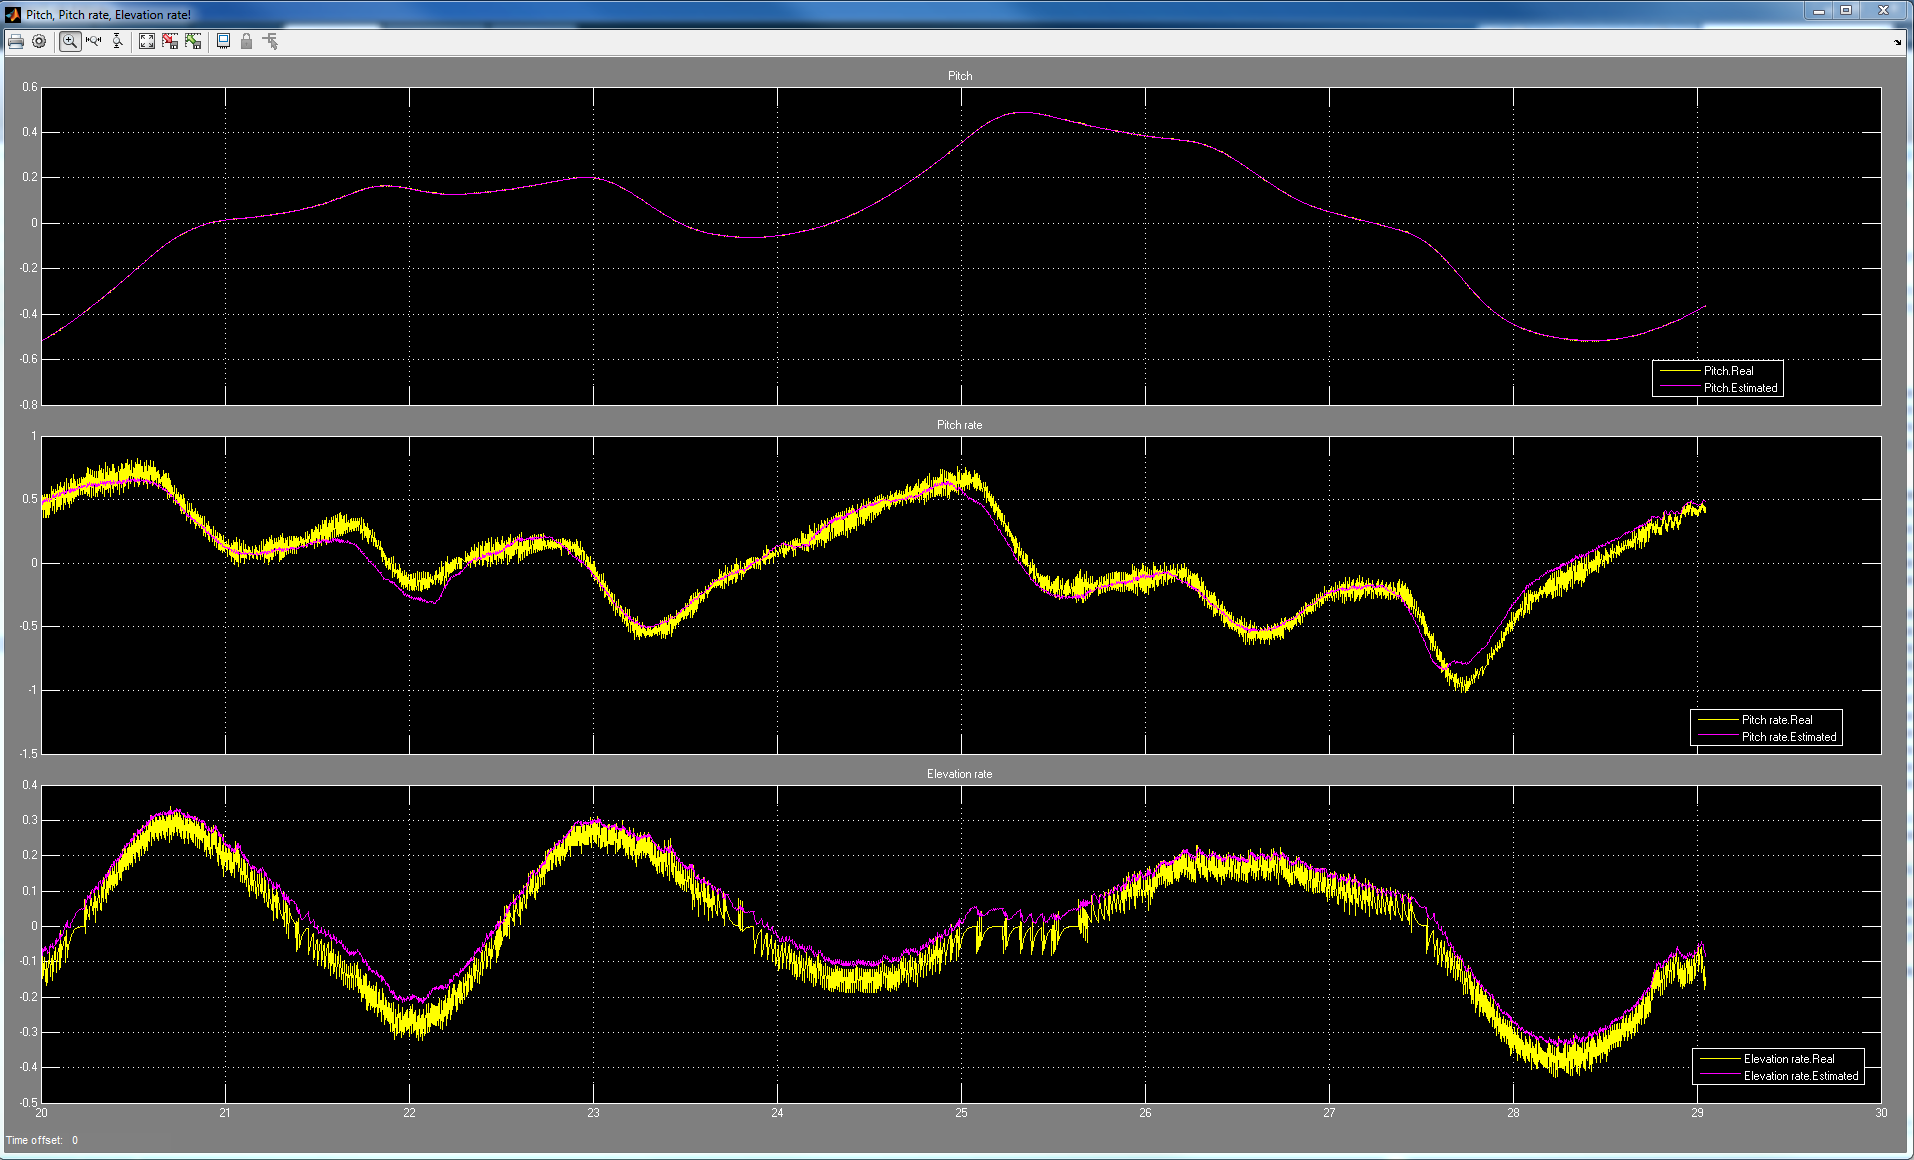
\includegraphics[width=1\textwidth]{figures/superplots_P4p2_del2_integrate_best.PNG}
	\caption{Part IV, problem 2 - PI controller. Shows the real (yellow) and estimated (purple) states for pitch, pitch rate and elevation rate respectively. Again, as we can see, the estimated states follows the real states quite well.}
\label{fig:P4p2_int_states_vs_obs}
\end{figure}
\begin{figure}[htb]
	\centering
		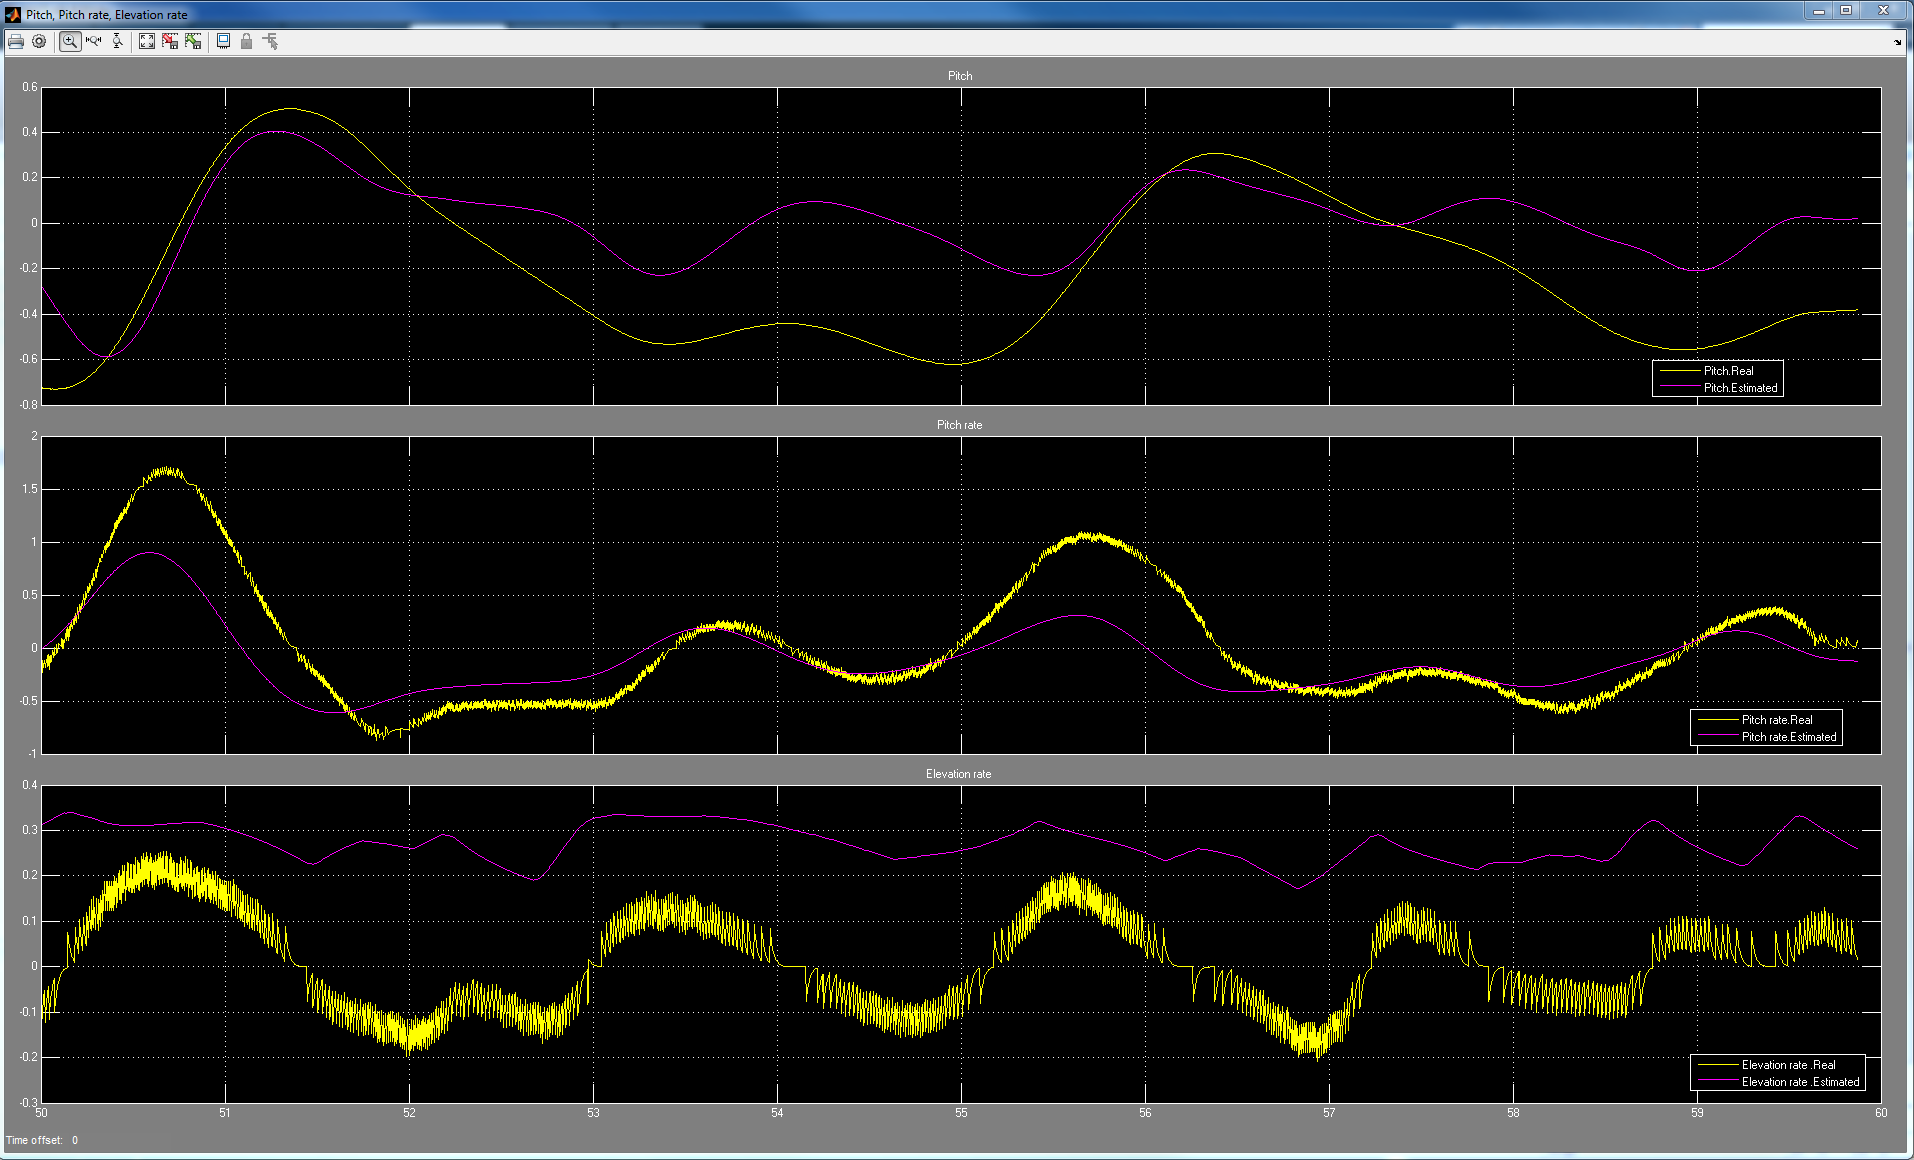
\includegraphics[width=1\textwidth]{figures/superplots_P4p3.PNG}
	\caption{Part IV, problem 3. Shows the real (yellow) and estimated (purple) states for pitch, pitch rate and elevation rate respectively. Clearly, this is not an optimal result as the real and estimated states differ quite a bit.}
\label{fig:P4p3}
\end{figure}
